\section{Futher Information}
\label{sec:04_furtherInformation}

\subsection{SNR}
\label{subsec:04_snr}

For the team filter, it the validity a robot result is useful information.
Depending on the uncertainty, the covariance of the incoming result can be adjusted.
Thus, one intuitive hypothesis is assuming the existence of a relation between the
received signal strength and distance to the source.
Taking the measurements of \ref{subsec:04_labMeasurements}, this hypothesis is
investigated by looking at the distance between one robot and the sound source.
According to this distance, it is looked at the \ac{SNR} of one measurement on
one robot proportional to all robots' \acp{SNR} of this measurement.
The \ac{SNR} on a single robot consists of the mean over all microphones' \acp{SNR}.
We can see in \cref{fig:04_snrDistance} that there is no straightforward
link between both values.
Also only taking a frame of size 256 samples into consideration
does not change the result.
% -------------------------------------------------------------
\begin{figure}[ht]
	\centering
	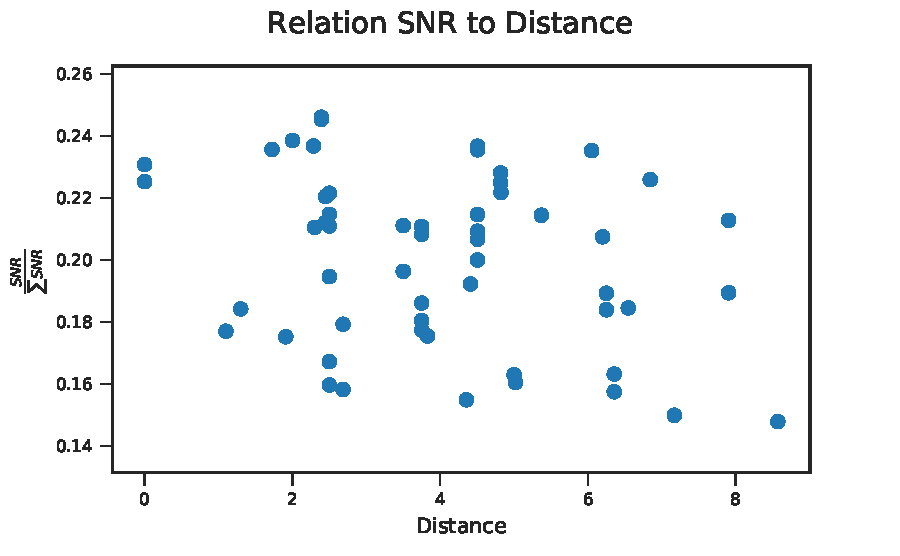
\includegraphics[]{figures/evaluation/snr_scatter}
	\caption{Visualization of relation between SNR and distance.}
	\label{fig:04_snrDistance}
\end{figure}
% -------------------------------------------------------------

Due to the unexpected result, further analysis on the \ac{SNR} values
on individual robots are done.
Therefore, a sine signal with fixed distance to the robot
was recorded from different angles with constant volume.
The main purpose of this measurement is to ensure that the lone channels
are not biased somehow.
Resulting from 14 measurements of a 3\si{\kilo\hertz} sine signal
with are distance of 0.73\si{m}, no tendency could be detected.
Further evaluation is done by determining the channel with the maximum
\ac{SNR} of one measurement. At 85,71\si{\percent} of the cases,
result coincided with the expected channel.
From this, we can say that the general recordings of the microphones
are neither biased nor falsified.

The same investigation is done with the real whistle recordings of the
measurement in \ref{subsec:04_labMeasurements}.
With these measurements only 54,55\si{\percent} of the maximum \acp{SNR}
match with the expected channels.
Consequentially, we must assume that the environmental circumstances
like multi-path propagation and reflection have large influence
on the signal magnitude.

\subsection{PSNR}
\label{subsec:04_psnr}

As referred in \cref{sec:02_gcc}, one characteristic of the \ac{GCC-PHAT}
algorithm is the sharp peak.
In conclusion, one can assume that if no sharp peak can be detected the
delay result of the \ac{GCC} has less informative value.
The validity of this statement is tested by comparing the \ac{PSNR} value
to the error of the direction angle resulting from the \ac{GCC-PHAT} delay.
Two cases of errors are taken into consideration.
In both, the \ac{PSNR} is recorded as high if it exceeds 17,5 whereat the
\ac{PSNR} value ranges from 10,1 to 28,8.

Firstly, each channel pair on one robot is looked at by determining the
smaller error between the actual angle and one of both direction candidates.
If the \ac{PSNR} of the \ac{GCC} is greater than the threshold of 17,5,
the \ac{RMSE} of its result is grouped to the errors with high \ac{PSNR}.
Elsewise it pertains to the errors with low \ac{PSNR}.
This valuation is done with the measurements of \cref{subsec:04_labMeasurements}
and manually set start indexes.
Having 76 correlations assessed with low \ac{PSNR}, the \ac{RMSE} of these
is 35,77\si{\degree}.
Compared to this, the \ac{RMSE} of the remaining 144 measurements
is 15,86\si{\degree}.

To see the impact on a complete robot result, the same is done
with the final errors on single robots.
Here, the \ac{RMSE} of the lower \ac{PSNR} case results in 25,36\si{\degree}
whereat the error of the other case is 14,41\si{\degree}.

From this, one can identify the \ac{PSNR} as valid additional information
for the covariance of a \ac{GCC-PHAT} delay result that enriches the
outcome of a robot direction ray that proceeds into the team filter.

Another option is to include the PSNR information into the single
robot whistle direction determination.
In \cref{fig:04_psnr2FrameShift}, the frame to investigate is
shifted multiple times before and after the signal start index
for the same measurement as in \cref{sec:04_tdoaSingle}.
There the robot was positioned at the center point
while the whistle was blown at -33,7\si{\degree} with 4,5\si{\meter}
distance.
The frame size of the \ac{GCC} is set to 256 samples and the shift
was set to a quarter of the frame size.
Samples of the rear left channel are plotted for better understanding.
The second graph shows the \ac{RMSE} of the single robot result
over the frame shifts.
For the lower graph, the mean over the \acp{PSNR} of all channels
is presented.
At zero shift, the start of the frame is set 50 samples previous to the
manually defined start index.
One sees, how the error is low with high \ac{PSNR} what confirms
the previous statement in this subsection.
For shifts smaller than -2, the signal is not represented in the
frames yet what explains the high error.
An important notice is that the result changes with proceeding
frames.
Without additional information about the rough direction,
ambiguity exists due to periodicity of the signal.
Due to the inconclusive result of the \ac{SNR} in \cref{subsec:04_snr}
one decides not to take the signal magnitude as such information
into account.
Thus, the decisive role of the start of the signal is underlined again.
% -------------------------------------------------------------
\begin{figure}[ht]
	\centering
	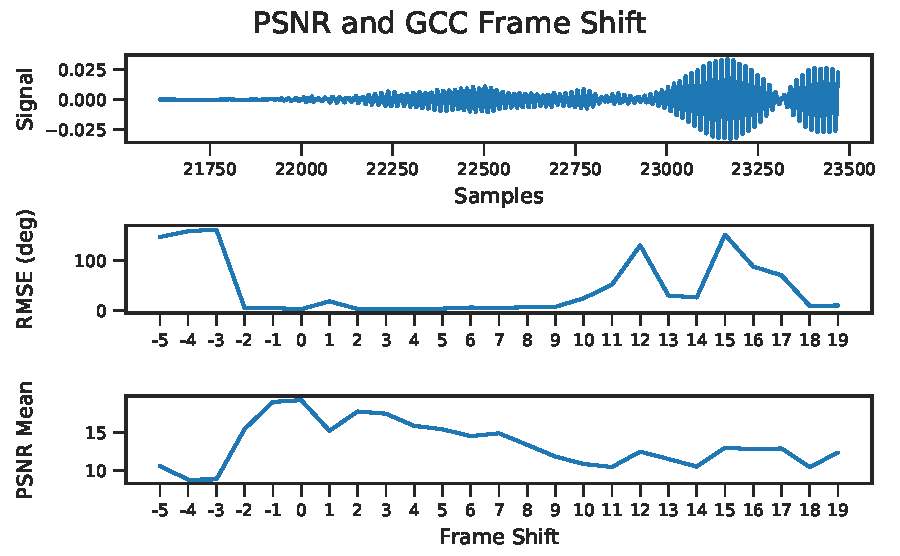
\includegraphics[]{figures/evaluation/gcc_frame_shift}
	\caption{
		Relation between \ac{PSNR} of correlation between channel 0 and 1
		and selection of the frame in time. Signal data
		of channel 0 on robot 26 is plotted for in the upper window.
		In this measurement, the whistle is positioned at measurement point 1
		of \cref{subsec:04_labMeasurements}.
	}
	\label{fig:04_psnr2FrameShift}
\end{figure}
% -------------------------------------------------------------


